\documentclass[xcolor=table, hyperref={pdfpagelabels=false}]{beamer}

\usepackage{amssymb}
\usepackage{lmodern}
\usepackage{animate}
\usepackage{pgfplots} 
\usepackage{tikz}
\usetikzlibrary{positioning,arrows,shapes}

% Embedded animations in Beamer
% \documentclass[]{beamer}

% Required package
% \usepackage{animate}

\usepackage[utf8]{inputenc} % this is needed for german umlauts
\usepackage[ngerman]{babel} % this is needed for german umlauts
\usepackage[T1]{fontenc}    % this is needed for correct output of umlauts in pdf

\usepackage{verbatim}

% see http://deic.uab.es/~iblanes/beamer_gallery/index_by_theme.html
% \usetheme{Frankfurt}

\usetheme{Warsaw}
%\usefonttheme{professionalfonts}

\setbeamertemplate{caption}{\raggedright\insertcaption\par}

\addtobeamertemplate{navigation symbols}{}{%
    \usebeamerfont{footline}%
    \usebeamercolor[fg]{footline}%
    \hspace{1em}%
    \insertframenumber/\inserttotalframenumber
}

%\title[About Beamer] %optional
%{About the Beamer class in presentation making}

\author[Farhan(1905035) \\ Ishrak(1905045) \\ Anonto(1905050)]
{Farhan Tahmidul Karim\inst{1} \and Md Ishrak Ahsan\inst{2} \and \\ Riad Ahmed Anonto\inst{3}}

\institute[VFU] % (optional)
{
  \inst{1}%
  1905035
  \and
  \inst{2}%
  1905045
  \and 
  \inst{3}
  1905050 
  \and
  \inst{1,2,3}%
  Department of Computer Science and Technology,BUET
}

\logo{\includegraphics[height=1cm]{overleaf-logo}}

\title{Dynamic Time Warping}

\renewcommand<>\cellcolor[1]{\only#2{\beameroriginal\cellcolor{#1}}}

\date{}

\begin{document}

\begin{frame}
\titlepage
\end{frame}

\section{Introduction}
\setbeamercovered{transparent}
\begin{frame}{What is Dynamic Time Warping?}
    \textit{\textbf{\Large{\textcolor{blue}{Dynamic Time Warping} is }} }
    \begin{itemize}
    \onslide<1->{\item \large{An algorithm used for measuring the similarity between two temporal time series sequence }}
    \onslide<2->{\item \large{Computes the distance from the matching similar elements between two series}}
    \onslide<3->{\item \large{Used in dynamic programming to find the optimal path}}
    \end{itemize}

\end{frame}

\setbeamercovered{invisible}
\begin{frame}{Motivation for DTW}
    \textbf{\Large{Tells us basically two things :}} 
    \begin{itemize}
    \onslide<1->{\item \large{How \textcolor{blue}{similar} are two signals }}
    \onslide<2->{\item \large{Which \textcolor{blue}{points correspond to} one another}}
    \end{itemize}

\end{frame}


\setbeamercovered{transparent}

\begin{frame}{So How do you figure out how similar the Signals are?}
\begin{block}{First Approach}
    \textcolor{blue}{\textbf{Euclidean Matching :}}\\
    Compare the \textcolor{blue}{Signals} point by point\\ \\
    \onslide<2->\textit{In fact, this approach is called the "Naive Approach"}
\end{block}    
\end{frame}

\begin{frame}{So How do you figure out how similar the Signals are?}
\begin{block}{Second Approach}
    \textcolor{blue}{\textbf{Dynamic Time Warping :}}\\
    Used for two \textcolor{blue}{variable-length arrays or time sequences} to create the best possible alignment. \\ \\ 
    \onslide<2->\textit{Exploiting the temporal distortions between them.}
\end{block}    
\end{frame}

\pgfdeclarelayer{background}
\pgfdeclarelayer{foreground}
\pgfsetlayers{background,main,foreground}


% \begin{frame}{GIFs in Beamer}
% \centering
% \animategraphics[loop,width=8cm]{10}{Chandler-}{0}{44}
% \end{frame}

\begin{frame}{Similarity Detection}
\centering
\animategraphics[width=8cm]{50}{Two_repeti-}{0}{154}
\end{frame}


\begin{frame}{Euclidean Matching Vs Dynamic Time Warping}
\begin{figure}
    \begin{tikzpicture}[]
        % Draw the vertices.
        \node (1) [red] at (-4,1) {\textbullet};
        \node (2) [red] at (-3,1) {\textbullet};
        \node (3) [red] at (-2,2) {\textbullet};
        \node (4) [red] at (-1,2) {\textbullet};
        \node (5) [red] at (0,1) {\textbullet};
        \node (6) [red] at (1,1) {\textbullet};
        \node (7) [red] at (2,0) {\textbullet};
        \node (8) [red] at (3,1) {\textbullet};
        \node (9) [red] at (4,1) {\textbullet};
        \node (10) [red] at (5,1) {\textbullet};
        \node (11) [red] at (6,1) {\textbullet};


        \node (12) [blue] at (-4,-2) {\textbullet};
        \node (13) [blue] at (-3,-2) {\textbullet};
        \node (14) [blue] at (-2,-2) {\textbullet};
        \node (15) [blue] at (-1,-2) {\textbullet};
        \node (16) [blue] at (0,-1) {\textbullet};
        \node (17) [blue] at (1,-1) {\textbullet};
        \node (18) [blue] at (2,-2) {\textbullet};
        \node (19) [blue] at (3,-2) {\textbullet};
        \node (20) [blue] at (4,-2) {\textbullet};
        \node (21) [blue] at (5,-3) {\textbullet};
        \node (22) [blue] at (6,-2.5) {\textbullet};
        \node (23) [blue] at (7,-2) {\textbullet};

        % Connect vertices with edges and draw weights
        \draw[line width=0.25mm, red] (-4,1)--(-3,1);
        \draw[line width=0.25mm,red] (-3,1)--(-2,2);
        \draw[line width=0.25mm,red] (-2,2)--(-1,2);
        \draw[line width=0.25mm,red] (-1,2)--(0,1);
        \draw[line width=0.25mm,red] (0,1)--(1,1);
        \draw[line width=0.25mm,red] (1,1)--(2,0);
        \draw[line width=0.25mm,red] (2,0)--(3,1);
        \draw[line width=0.25mm,red] (3,1)--(4,1);
        \draw[line width=0.25mm,red] (4,1)--(5,1);
        \draw[line width=0.25mm,red] (5,1)--(6,1);


        \draw[line width=0.25mm, blue] (-4,-2)--(-3,-2);
        \draw[line width=0.25mm,blue] (-3,-2)--(-2,-2);
        \draw[line width=0.25mm,blue] (-2,-2)--(-1,-2);
        \draw[line width=0.25mm,blue] (-1,-2)--(0,-1);
        \draw[line width=0.25mm,blue] (0,-1)--(1,-1);
        \draw[line width=0.25mm,blue] (1,-1)--(2,-2);
        \draw[line width=0.25mm,blue] (2,-2)--(3,-2);
        \draw[line width=0.25mm,blue] (3,-2)--(4,-2);
        \draw[line width=0.25mm,blue] (4,-2)--(5,-3);
        \draw[line width=0.25mm,blue] (5,-3)--(6,-2.5);
        \draw[line width=0.25mm,blue] (6,-2.5)--(7,-2);
        
        % \path [red] (1) edge node {} (2);
     

        \begin{pgfonlayer}{background}
            \path<2-5>[draw,line width=0.5mm,-,black!50] (1.center) edge node {} (12.center);
            \path<3-5>[draw,line width=0.5mm,-,black!50] (2.center) edge node {} (13.center);
            \path<5-5>[draw,line width=0.5mm,-,black!50] (3.center) edge node {} (14.center);
            \path<5-5>[draw,line width=0.5mm,-,black!50] (4.center) edge node {} (15.center);
            \path<5-5>[draw,line width=0.5mm,-,black!50] (5.center) edge node {} (16.center);
            \path<5-5>[draw,line width=0.5mm,-,black!50] (6.center) edge node {} (17.center);
            \path<5-5>[draw,line width=0.5mm,-,black!50] (7.center) edge node {} (18.center);
            \path<5-5>[draw,line width=0.5mm,-,black!50] (8.center) edge node {} (19.center);
            \path<5-5>[draw,line width=0.5mm,-,black!50] (9.center) edge node {} (20.center);
            \path<5-5>[draw,line width=0.5mm,-,black!50] (10.center) edge node {} (21.center);
            \path<5-5>[draw,line width=0.5mm,-,black!50] (11.center) edge node {} (22.center);
            % \path<10->[draw,line width=5pt,-,red!50] (b.center) edge node {} (d.center);
            % \path<12->[draw,line width=5pt,-,red!50] (d.center) edge node {} (e.center);

            \node<4-5> (x1) [above of = 1, yshift = -0.5cm] {$x_1$};
            \node<4-5> (x2) [above of = 2, yshift = -0.5cm] {$x_2$};
            \node<4-5> (y1) [below of = 12, yshift = 0.5cm] {$y_1$};
            \node<4-5> (y2) [below of = 13, yshift = 0.5cm] {$y_2$};

            \node<5-5> (xn) [above of = 11, yshift = -0.5cm] {$x_n$};
            \node<5-5> (yn) [below of = 22, yshift = 0.5cm] {$y_n$};
            

            % \path<6-6>[draw,line width=0.5mm,-,black!50] (1.center) edge node {} (12.center);
            % \path<6-6>[draw,line width=0.5mm,-,black!50] (1.center) edge node {} (13.center);
            % \path<6-6>[draw,line width=0.5mm,-,black!50] (1.center) edge node {} (14.center);
            % \path<6-6>[draw,line width=0.5mm,-,black!50] (2.center) edge node {} (15.center);
            % \path<6-6>[draw,line width=0.5mm,-,black!50] (3.center) edge node {} (16.center);
            % \path<6-6>[draw,line width=0.5mm,-,black!50] (4.center) edge node {} (17.center);
            % \path<6-6>[draw,line width=0.5mm,-,black!50] (5.center) edge node {} (18.center);
            % \path<6-6>[draw,line width=0.5mm,-,black!50] (6.center) edge node {} (19.center);
            % \path<6-6>[draw,line width=0.5mm,-,black!50] (7.center) edge node {} (20.center);
            % \path<6-6>[draw,line width=0.5mm,-,black!50] (8.center) edge node {} (21.center);
            % \path<6-6>[draw,line width=0.5mm,-,black!50] (9.center) edge node {} (22.center);
            % \path<6-6>[draw,line width=0.5mm,-,black!50] (10.center) edge node {} (22.center);
            % \path<6-6>[draw,line width=0.5mm,-,black!50] (11.center) edge node {} (23.center);

        \end{pgfonlayer}
    \end{tikzpicture}
   
\end{figure}
\end{frame}

\begin{frame}{Euclidean Matching Vs Dynamic Time Warping}
\begin{figure}
    \begin{tikzpicture}[]
        % Draw the vertices.
        \node (1) [red] at (-4,1) {\textbullet};
        \node (2) [red] at (-3,1) {\textbullet};
        \node (3) [red] at (-2,2) {\textbullet};
        \node (4) [red] at (-1,2) {\textbullet};
        \node (5) [red] at (0,1) {\textbullet};
        \node (6) [red] at (1,1) {\textbullet};
        \node (7) [red] at (2,0) {\textbullet};
        \node (8) [red] at (3,1) {\textbullet};
        \node (9) [red] at (4,1) {\textbullet};
        \node (10) [red] at (5,1) {\textbullet};
        \node (11) [red] at (6,1) {\textbullet};


        \node (12) [blue] at (-4,-2) {\textbullet};
        \node (13) [blue] at (-3,-2) {\textbullet};
        \node (14) [blue] at (-2,-2) {\textbullet};
        \node (15) [blue] at (-1,-2) {\textbullet};
        \node (16) [blue] at (0,-1) {\textbullet};
        \node (17) [blue] at (1,-1) {\textbullet};
        \node (18) [blue] at (2,-2) {\textbullet};
        \node (19) [blue] at (3,-2) {\textbullet};
        \node (20) [blue] at (4,-2) {\textbullet};
        \node (21) [blue] at (5,-3) {\textbullet};
        \node (22) [blue] at (6,-2.5) {\textbullet};
        \node (23) [blue] at (7,-2) {\textbullet};

        % Connect vertices with edges and draw weights
        \draw[line width=0.25mm, red] (-4,1)--(-3,1);
        \draw[line width=0.25mm,red] (-3,1)--(-2,2);
        \draw[line width=0.25mm,red] (-2,2)--(-1,2);
        \draw[line width=0.25mm,red] (-1,2)--(0,1);
        \draw[line width=0.25mm,red] (0,1)--(1,1);
        \draw[line width=0.25mm,red] (1,1)--(2,0);
        \draw[line width=0.25mm,red] (2,0)--(3,1);
        \draw[line width=0.25mm,red] (3,1)--(4,1);
        \draw[line width=0.25mm,red] (4,1)--(5,1);
        \draw[line width=0.25mm,red] (5,1)--(6,1);


        \draw[line width=0.25mm, blue] (-4,-2)--(-3,-2);
        \draw[line width=0.25mm,blue] (-3,-2)--(-2,-2);
        \draw[line width=0.25mm,blue] (-2,-2)--(-1,-2);
        \draw[line width=0.25mm,blue] (-1,-2)--(0,-1);
        \draw[line width=0.25mm,blue] (0,-1)--(1,-1);
        \draw[line width=0.25mm,blue] (1,-1)--(2,-2);
        \draw[line width=0.25mm,blue] (2,-2)--(3,-2);
        \draw[line width=0.25mm,blue] (3,-2)--(4,-2);
        \draw[line width=0.25mm,blue] (4,-2)--(5,-3);
        \draw[line width=0.25mm,blue] (5,-3)--(6,-2.5);
        \draw[line width=0.25mm,blue] (6,-2.5)--(7,-2);
        
        % \path [red] (1) edge node {} (2);
     

        \begin{pgfonlayer}{background}
            \path<1-1>[draw,line width=0.5mm,-,black!50] (1.center) edge node {} (12.center);
            \path<1-1>[draw,line width=0.5mm,-,black!50] (2.center) edge node {} (13.center);
            \path<1-1>[draw,line width=0.5mm,-,black!50] (3.center) edge node {} (14.center);
            \path<1-1>[draw,line width=0.5mm,-,black!50] (4.center) edge node {} (15.center);
            \path<1-1>[draw,line width=0.5mm,-,black!50] (5.center) edge node {} (16.center);
            \path<1-1>[draw,line width=0.5mm,-,black!50] (6.center) edge node {} (17.center);
            \path<1-1>[draw,line width=0.5mm,-,black!50] (7.center) edge node {} (18.center);
            \path<1-1>[draw,line width=0.5mm,-,black!50] (8.center) edge node {} (19.center);
            \path<1-1>[draw,line width=0.5mm,-,black!50] (9.center) edge node {} (20.center);
            \path<1-1>[draw,line width=0.5mm,-,black!50] (10.center) edge node {} (21.center);
            \path<1-1>[draw,line width=0.5mm,-,black!50] (11.center) edge node {} (22.center);
            % \path<10->[draw,line width=5pt,-,red!50] (b.center) edge node {} (d.center);
            % \path<12->[draw,line width=5pt,-,red!50] (d.center) edge node {} (e.center);

            \node<1-1> (x1) [above of = 1, yshift = -0.5cm] {$x_1$};
            \node<1-1> (x2) [above of = 2, yshift = -0.5cm] {$x_2$};
            \node<1-1> (y1) [below of = 12, yshift = 0.5cm] {$y_1$};
            \node<1-1> (y2) [below of = 13, yshift = 0.5cm] {$y_2$};

            \node<1-1> (xn) [above of = 11, yshift = -0.5cm] {$x_n$};
            \node<1-1> (yn) [below of = 22, yshift = 0.5cm] {$y_n$};
            

        \end{pgfonlayer}
    \end{tikzpicture}
   
\end{figure}

Formula can be written as :
\begin{equation}    
     d(x_1_:_N,y_1_:_M) = \sum_{i=1}^n |x_i-y_i|
\end{equation}

\end{frame}

\begin{frame}{Euclidean Matching Vs Dynamic Time Warping}
\begin{figure}
    \begin{tikzpicture}[]
        % Draw the vertices.
        \node (1) [red] at (-4,1) {\textbullet};
        \node (2) [red] at (-3,1) {\textbullet};
        \node (3) [red] at (-2,2) {\textbullet};
        \node (4) [red] at (-1,2) {\textbullet};
        \node (5) [red] at (0,1) {\textbullet};
        \node (6) [red] at (1,1) {\textbullet};
        \node (7) [red] at (2,0) {\textbullet};
        \node (8) [red] at (3,1) {\textbullet};
        \node (9) [red] at (4,1) {\textbullet};
        \node (10) [red] at (5,1) {\textbullet};
        \node (11) [red] at (6,1) {\textbullet};


        \node (12) [blue] at (-4,-2) {\textbullet};
        \node (13) [blue] at (-3,-2) {\textbullet};
        \node (14) [blue] at (-2,-2) {\textbullet};
        \node (15) [blue] at (-1,-2) {\textbullet};
        \node (16) [blue] at (0,-1) {\textbullet};
        \node (17) [blue] at (1,-1) {\textbullet};
        \node (18) [blue] at (2,-2) {\textbullet};
        \node (19) [blue] at (3,-2) {\textbullet};
        \node (20) [blue] at (4,-2) {\textbullet};
        \node (21) [blue] at (5,-3) {\textbullet};
        \node (22) [blue] at (6,-2.5) {\textbullet};
        \node (23) [blue] at (7,-2) {\textbullet};

        % Connect vertices with edges and draw weights
        \draw[line width=0.25mm, red] (-4,1)--(-3,1);
        \draw[line width=0.25mm,red] (-3,1)--(-2,2);
        \draw[line width=0.25mm,red] (-2,2)--(-1,2);
        \draw[line width=0.25mm,red] (-1,2)--(0,1);
        \draw[line width=0.25mm,red] (0,1)--(1,1);
        \draw[line width=0.25mm,red] (1,1)--(2,0);
        \draw[line width=0.25mm,red] (2,0)--(3,1);
        \draw[line width=0.25mm,red] (3,1)--(4,1);
        \draw[line width=0.25mm,red] (4,1)--(5,1);
        \draw[line width=0.25mm,red] (5,1)--(6,1);


        \draw[line width=0.25mm, blue] (-4,-2)--(-3,-2);
        \draw[line width=0.25mm,blue] (-3,-2)--(-2,-2);
        \draw[line width=0.25mm,blue] (-2,-2)--(-1,-2);
        \draw[line width=0.25mm,blue] (-1,-2)--(0,-1);
        \draw[line width=0.25mm,blue] (0,-1)--(1,-1);
        \draw[line width=0.25mm,blue] (1,-1)--(2,-2);
        \draw[line width=0.25mm,blue] (2,-2)--(3,-2);
        \draw[line width=0.25mm,blue] (3,-2)--(4,-2);
        \draw[line width=0.25mm,blue] (4,-2)--(5,-3);
        \draw[line width=0.25mm,blue] (5,-3)--(6,-2.5);
        \draw[line width=0.25mm,blue] (6,-2.5)--(7,-2);
        
        % \path [red] (1) edge node {} (2);
     

        \begin{pgfonlayer}{background}
            

            \path<1-1>[draw,line width=0.5mm,-,black!50] (1.center) edge node {} (12.center);
            \path<1-1>[draw,line width=0.5mm,-,black!50] (1.center) edge node {} (13.center);
            \path<1-1>[draw,line width=0.5mm,-,black!50] (1.center) edge node {} (14.center);
            \path<1-1>[draw,line width=0.5mm,-,black!50] (2.center) edge node {} (15.center);
            \path<1-1>[draw,line width=0.5mm,-,black!50] (3.center) edge node {} (16.center);
            \path<1-1>[draw,line width=0.5mm,-,black!50] (4.center) edge node {} (17.center);
            \path<1-1>[draw,line width=0.5mm,-,black!50] (5.center) edge node {} (18.center);
            \path<1-1>[draw,line width=0.5mm,-,black!50] (6.center) edge node {} (19.center);
            \path<1-1>[draw,line width=0.5mm,-,black!50] (7.center) edge node {} (20.center);
            \path<1-1>[draw,line width=0.5mm,-,black!50] (8.center) edge node {} (21.center);
            \path<1-1>[draw,line width=0.5mm,-,black!50] (9.center) edge node {} (22.center);
            \path<1-1>[draw,line width=0.5mm,-,black!50] (10.center) edge node {} (22.center);
            \path<1-1>[draw,line width=0.5mm,-,black!50] (11.center) edge node {} (23.center);

        \end{pgfonlayer}
    \end{tikzpicture}
   
\end{figure}
\end{frame}

\begin{frame}{Dynamic Time Warping}
   
\begin{center}
  \begin{tabular}{|c|c|}
    \hline
    \begin{minipage}{0.3\textwidth}
      \centering
      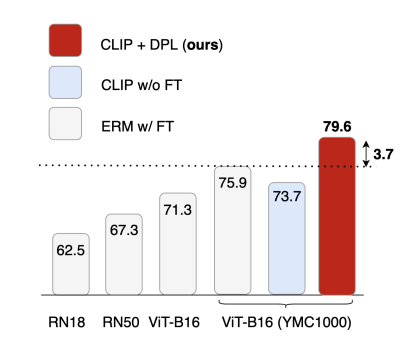
\includegraphics[width=\linewidth]{1.png}
    \end{minipage}
    &
    \begin{minipage}{0.6\textwidth}
      \centering
      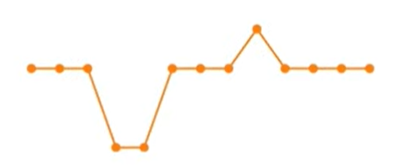
\includegraphics[width=0.3\linewidth]{2.png}
      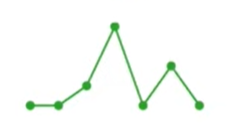
\includegraphics[width=0.3\linewidth]{3.png}
    \end{minipage}
    \\
    \hline
  \end{tabular}
\end{center}

% \begin{figure}
%     \centering
%     \begin{subfigure}{\textwidth}
%      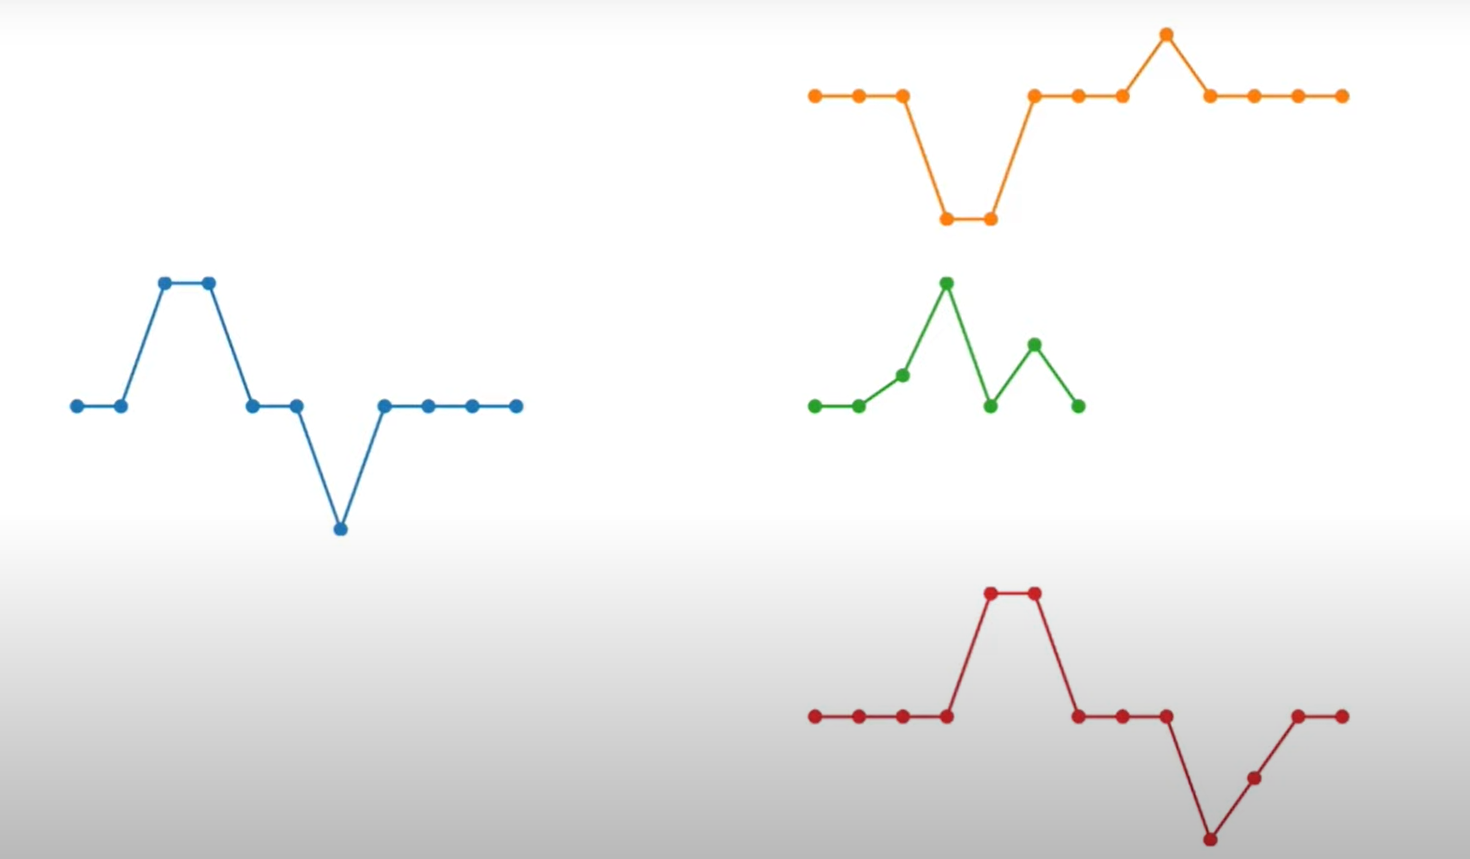
\includegraphics[width = \linewidth]{d.p}
%     \label{fig:my_label}
%     \end{subfigure}
% \end{figure}

\end{frame}


\begin{frame}{How DTW is Different?}
\begin{columns}
\column{0.5\textwidth}
\large{\textbf{Euclidean Matching}}
\begin{itemize}
    \item[$\checkmark$] One to one point Comparison 
    \item[$\checkmark$] That's why compares only time series of same length 
\end{itemize}

\column{0.5\textwidth}
\large{\textbf{Dynamic Time Warping}}
\begin{itemize}
    \item[$\checkmark$] Allows many-to-one comparisons 
    \item[$\checkmark$] Time series of different length can be compared
\end{itemize}
    
\end{columns} 
\end{frame}

\section{Implementation}

\begin{frame}{Algorithm}

int DTWDistance(s: array [1..n], t: array [1..m]) \{ \\
    \quad DTW := array [0..n, 0..m] \\
    
    \quad for i := 0 to n \\
        \quad \quad for j := 0 to m \\
            \quad \quad \quad DTW[i, j] := \infty \\
    \quad DTW[0, 0] := 0 \\
    
    \quad for i := 1 to n \\
        \quad \quad for j := 1 to m \\
            \quad \quad \quad cost := d(s[i], t[j]) \\
            \quad \quad \quad DTW[i, j] := cost + min(DTW[i-1, j],    // insertion \\
                                       \quad \quad \quad \quad \quad \quad \quad \quad \quad \quad \quad \quad \quad \quad DTW[i, j-1],    // deletion \\
                                        \quad \quad \quad \quad \quad \quad \quad \quad \quad \quad \quad \quad \quad \quad DTW[i-1, j-1])    // match \\
    
    \quad return DTW[n, m] \\
\}

\end{frame}

\begin{frame}{Distance Matrix}
    
Let us consider two time series \pause \newline
\begin{equation*}
    TS_A = [1, 3, 4, 9, 8, 2] 
\end{equation*}
\begin{equation*}
    TS_B = [1, 6, 2, 3, 0, 9, 4]
\end{equation*}
\end{frame}

\begin{frame}{Distance Matrix}
    \begin{center}
        \begin{tabular}{ c | c | c | c | c | c | c | c | }
           \cline{2-8}
           2 & \onslide<13->{\cellcolor<13>{yellow}21} & \onslide<13->{\cellcolor<13>{yellow}13} & \onslide<13->{\cellcolor<13>{yellow}9} & \onslide<13->{\cellcolor<13>{yellow}10} & \onslide<13->{\cellcolor<13>{yellow}12} & \onslide<13->{\cellcolor<13>{yellow}16} & \onslide<13->{\cellcolor<13>{yellow}11} \\ \cline{2-8}
           8 & \onslide<13->{\cellcolor<13>{yellow}20} & \onslide<13->{\cellcolor<13>{yellow}9} & \onslide<13->{\cellcolor<13>{yellow}13} & \onslide<13->{\cellcolor<13>{yellow}16} & \onslide<13->{\cellcolor<13>{yellow}19} & \onslide<13->{\cellcolor<13>{yellow}9} & \onslide<13->{\cellcolor<13>{yellow}12} \\ \cline{2-8}
           \cellcolor<12>{lightgray}9 & \onslide<11->{\cellcolor<11>{yellow}13} & \onslide<11->{\cellcolor<11>{yellow}7} & \onslide<11->{\cellcolor<11>{yellow}11} & \onslide<11->{\cellcolor<11>{yellow}\cellcolor<12>{pink}11} & \onslide<12->{\cellcolor<12>{yellow}14} & \onslide<13->{\cellcolor<13>{yellow}8} & \onslide<13->{\cellcolor<13>{yellow}13} \\ \cline{2-8}
           \cellcolor<9>{lightgray}4 & \onslide<9->{\cellcolor<9>{yellow}5} & \onslide<10->{\cellcolor<10>{yellow}4} & \onslide<10->{\cellcolor<10>{yellow}5} & \onslide<10->{\cellcolor<10>{yellow}\cellcolor<12>{pink}5} & \onslide<10->{\cellcolor<10>{yellow}\cellcolor<12>{pink}8} & \onslide<10->{\cellcolor<10>{yellow}12} & \onslide<10->{\cellcolor<10>{yellow}12} \\ \cline{2-8}
           \cellcolor<6,7>{lightgray}3 & \onslide<6->{\cellcolor<6>{yellow}\cellcolor<7,9>{pink}2} & \onslide<7->{\cellcolor<7>{yellow}3} & \onslide<8->{\cellcolor<8>{yellow}4} & \onslide<8->{\cellcolor<8>{yellow}4} & \onslide<8->{\cellcolor<8>{yellow}7} & \onslide<8->{\cellcolor<8>{yellow}12} & \onslide<8->{\cellcolor<8>{yellow}14} \\ \cline{2-8}
           \cellcolor<2,3,4>{lightgray}1 & \onslide<2->{\cellcolor<2>{yellow}\cellcolor<3,6,7>{pink}0} & \onslide<3->{\cellcolor<3>{yellow}\cellcolor<4,7>{pink}5} & \onslide<4->{\cellcolor<4>{yellow}6} & \onslide<5->{\cellcolor<5>{yellow}8} & \onslide<5->{\cellcolor<5>{yellow}9} & \onslide<5->{\cellcolor<5>{yellow}17} & \onslide<5->{\cellcolor<5>{yellow}20} \\ \cline{2-8}
           \multicolumn{1}{c}{} & \multicolumn{1}{c}{\cellcolor<2,6,9>{lightgray}1} & \multicolumn{1}{c}{\cellcolor<3,7>{lightgray}6} & \multicolumn{1}{c}{\cellcolor<4>{lightgray}2} & \multicolumn{1}{c}{3} & \multicolumn{1}{c}{\cellcolor<12>{lightgray}0} & \multicolumn{1}{c}{9} & \multicolumn{1}{c}{4}
        \end{tabular}
    \end{center}

    \begin{equation*}
        D_{i, j} = |A_i - B_j| + min(D_{i-1, j-1}, D_{i-1, j}, D_{i, j-1})
    \end{equation*}
    
\end{frame}

\begin{frame}{Optimal Path}
    \begin{center}
        \begin{tabular}{ c | c | c | c | c | c | c | c | }
           \cline{2-8}
           2 & 21 & 13 & 9 & 10 & 12 & 16 & \cellcolor<2->{lightgray}11 \\ \cline{2-8}
           8 & 20 & 9 & 13 & 16 & 19 & \cellcolor<3->{lightgray}9 & 12 \\ \cline{2-8}
           9 & 13 & 7 & 11 & 11 & 14 & \cellcolor<4->{lightgray}8 & 13 \\ \cline{2-8}
           4 & 5 & 4 & 5 & 5 & \cellcolor<5->{lightgray}8 & 12 & 12 \\ \cline{2-8}
           3 & 2 & \cellcolor<8->{lightgray}3 & \cellcolor<7->{lightgray}4 & \cellcolor<6->{lightgray}4 & 7 & 13 & 14 \\ \cline{2-8}
           1 & \cellcolor<9->{lightgray}0 & 5 & 6 & 8 & 9 & 17 & 20 \\ \cline{2-8}
           \multicolumn{1}{c}{} & \multicolumn{1}{c}{1} & \multicolumn{1}{c}{6} & \multicolumn{1}{c}{2} & \multicolumn{1}{c}{3} & \multicolumn{1}{c}{0} & \multicolumn{1}{c}{9} & \multicolumn{1}{c}{4}
        \end{tabular}
    \end{center}

    \begin{enumerate}
        \item<1,2-2> Start at $D_{n, m}$
        \item<1,3-> Find $min(D_{i-1, j-1}, D_{i-1, j}, D_{i, j-1})$, add to current path and jump to that cell
        \item<1,4-> Proceed until we reach $D_{1, 1}$
    \end{enumerate}
\end{frame}

\section{Applications}

\begin{frame}{Applications of DTW}
    \begin{itemize}
    \item<1-> Spoken Word Recognition %C will appear in all slides of the list from 1
    \item<2-> Detect Sales \& Trend %C++ will come in only slides 2 and 3
    \item<3-> Wearable Fitness Trackers
    \item<4-> Route and ETA Calculation
\end{itemize}
    
\end{frame}

\begin{frame}{Spoken Word Recognition by Matching Sound Pattern}
    \begin{figure}
        \centering
        \begin{subfigure}{\textwidth}
            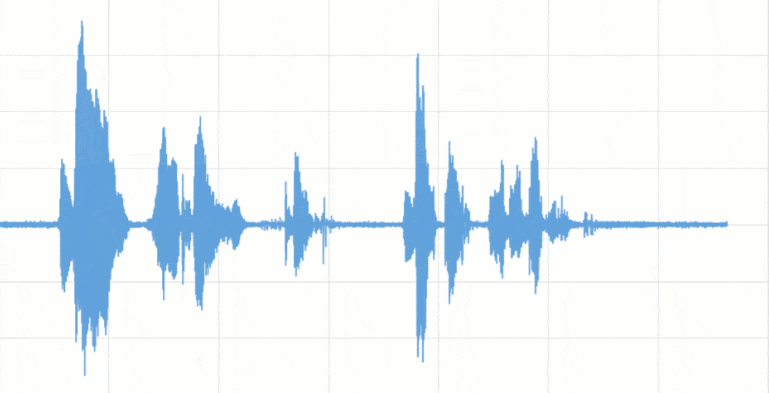
\includegraphics[width = 0.4\linewidth]{voice 1.png}
            \caption{"Doors and corners, kid. That's where they get you" - v1}
            \label{fig:my_label_1}
        \end{subfigure}
        \begin{subfigure}{\textwidth}
        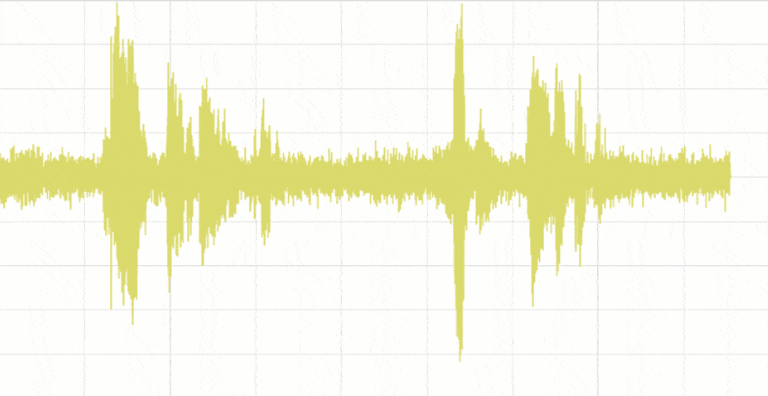
\includegraphics[width = 0.4\linewidth]{voice 2.png}
        \caption{"Doors and corners, kid. That's where they get you" - v2}
        \label{fig:my_label_2}
        \end{subfigure}
    \end{figure}
\end{frame}

% \tikzstyle{pinnode}=[circle,draw=grey!60,fill=grey!40,very thick, minimum size=3mm]

\begin{frame}{Spoken Word Recognition by Sound Matching Pattern: Euclidian Approach}
    \begin{figure}
        \centering
        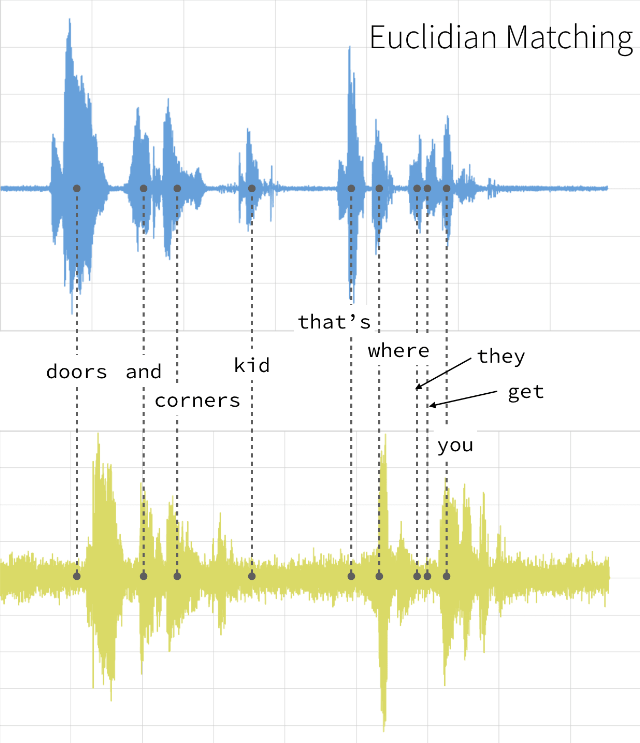
\includegraphics[width = 0.8\linewidth, height = 0.7\textheight]{EucMat.png}
        \caption{Failure of Euclidian matching in identifying speech delays/pauses}
        \label{fig:my_label_Euclid}
    \end{figure}
\end{frame}


\begin{frame}{Spoken Word Recognition by Sound Matching Pattern: Using DTW }
\centering
\animategraphics[loop,width=8cm]{2}{dtw-animated-}{0}{11}
\end{frame}

\begin{frame}
    \frametitle{Detecting Sales Trends}
    \begin{table}
    \centering
    \begin{tabular}{|s|p{2cm}|p{2cm}| p{1cm}| p{2cm}|}
        \hline
        \rowcolor{lightgray} \multicolumn{5}{|c|}{Units of each product sold per week} \\
        \hline
        \textbf{Product Code} &\textbf{W1} &\textbf{W2} &\textbf{\dots} &\textbf{W52} \\
        \hline
        \textbf{P1} &11 &12 &\dots &7 \\
        \textbf{P2} &7 &6 &\dots &4 \\
        \textbf{P3} &7 &11 &\dots &3 \\
        \textbf{P4} &12 &8 &\dots &2 \\
        \textbf{P5} &8 &5 &\dots &0 \\
        \textbf{P6} &4 &3 &\dots &10 \\
        \textbf{P7} &5 &6 &\dots &5 \\
        \textbf\dots &\dots &\dots &\dots &\dots \\
        \textbf{P20} &18 &6 &\dots  &7 \\
        \hline
    \end{tabular}
    \caption{\label{demo-table}Weekly sales transaction data set of a company throughout last year}
    \end{table}
\end{frame}

\begin{frame}
    \frametitle{Detecting Sales Trends}
    \begin{tikzpicture}
    \begin{axis} [
        title={DTW distances for each pairwise product sales comparison},
        ybar,
        height=7cm,
        width=0.8\paperwidth,
        axis lines = left,
        xlabel = \(Distances\),
        ylabel = {\(Counts\)},
    ]
        \addplot coordinates {
            (1,8.55) 
            (2,4.70) 
            (3,15.90) 
            (4,29.44)
            (5,32.66)
            (6,42.78)
            (7,57.89)
            (8,63.44)
            (9,80.37)
            (10,73.23)
            (11,82.4)
            (12,79.78)
            (13,75.99)
            (14,49.8)
            (15,45.12)
            (16,20.42)
            (17,8.76)
            (18,4.23)
            (19,5.28)
            (20,6.55)
        };
    \end{axis}
\end{tikzpicture}

\end{frame}

\begin{frame}
    \frametitle{Detecting Sales Trends}
    \begin{tikzpicture}
    \begin{axis} [
        title={Comparing Optimal Sales Trend with the Furthest and Closest Products},
        height=6cm,
        width=0.9\paperwidth,
        axis lines = left,
        xlabel = \(Week\),
        ylabel = {\(Sales\)},
        legend style={at={(5,-2)}}
    ]
        \addplot[
            color=blue,
            mark=*,
        ] coordinates {
            (1,12.5)
            (2,13)
            (3,13.5)
            (4,14.2)
            (5,17)
            (6,10)
            (7,15.1)
            (8,16)
            (9,17)
            (10,15.9)
            (11,19.2)
            (12,14.2)
            (13,14.2)
            (14,15)
            (15,10.9)
            (16,20)
            (17,17.8)
            (18,17)
            (19,19.1)
            (20,21)
            (21,19.5)
            (22,15.2)
            (23,16.2)
            (24,16.2)
            (25,15.8)
            (26,15.1)
            (27,19.2)
            (28,19.2)
            (29,20)
            (30,21)
            (31,19.1)
            (32,18)
            (33,17)
            (34,16)
            (35,20)
            (36,19)
            (37,19)
            (38,18)
            (39,17)
            (40,17.6)
            (41,26)
            (42,25)
            (43,16.2)
            (44,23)
            (45,20.8)
            (46,19.5)
            (47,28)
            (48,18)
            (49,19.2)
            (50,15.5)
            (51,21)
            (52,23)
        };
        \legend{Optimal Sales Trend}
        \addplot [
            color=green,
            mark=10-pointed star,
        ] coordinates {
            (1,2)
            (2,0.5)
            (3,4.5)
            (4,0)
            (5,2)
            (6,5)
            (7,5)
            (8,1)
            (9,3)
            (10,2.5)
            (11,1)
            (12,1)
            (13,1)
            (14,1)
            (15,8)
            (16,5)
            (17,3)
            (18,6)
            (19,3)
            (20,6)
            (21,7)
            (22,5)
            (23,4.2)
            (24,4.2)
            (25,10)
            (26,7)
            (27,3)
            (28,5)
            (29,7)
            (30,4.5)
            (31,4.5)
            (32,1)
            (33,2)
            (34,3)
            (35,5.8)
            (36,4.5)
            (37,5.8)
            (38,5.8)
            (39,5.8)
            (40,4.5)
            (41,8)
            (42,7.4)
            (43,7.4)
            (44,6)
            (45,5)
            (46,5)
            (47,5)
            (48,7)
            (49,7)
            (50,5)
            (51,9)
            (52,10)
        };
        \legend{Optimal Sales Trend, P18 (Closest to optimal)}
        \addplot [
            color=orange,
            mark=triangle,
        ] coordinates {
            (1,1)
            (2,0)
            (3,0)
            (4,0.5)
            (5,1.5)
            (6,0)
            (7,0)
            (8,0)
            (9,0)
            (10,1)
            (11,1.2)
            (12,1.4)
            (13,0.6)
            (14,0)
            (15,0)
            (16,0)
            (17,0)
            (18,0)
            (19,0)
            (20,0)
            (21,0.5)
            (22,2)
            (23,1.5)
            (24,1.1)
            (25,2.5)
            (26,0.5)
            (27,0)
            (28,3.4)
            (29,1)
            (30,1.2)
            (31,0.5)
            (32,0)
            (33,0)
            (34,2)
            (35,1.2)
            (36,1.1)
            (37,1.3)
            (38,1.9)
            (39,2)
            (40,0)
            (41,2.5)
            (42,1.2)
            (43,1)
            (44,0)
            (45,0)
            (46,0)
            (47,0)
            (48,1)
            (49,1)
            (50,1.5)
            (51,0)
            (52,0.4)
        };
        \legend{Optimal Sales Trend, P18 (Closest to optimal, P11 (Furthest to optimal)}
    \end{axis}
\end{tikzpicture}
    
\end{frame}

\begin{frame} 
    \begin{figure}
        \centering
        
\includegraphics[width = 0.9\linewidth, height = 0.7\textheight]{end.jpg}
        \label{fig:end}
    \end{figure}
\end{frame}

\end{document}
